\chapter{Estado del Arte}\label{chapter:state-of-the-art}

\section{M\'etodo del Desempate Instant\'aneo}
En los sistemas mayoritarios es necesario que un candidato alcance la mayor\'ia de votos (un determinado porcentaje de los votos) para obtener la victoria. Si esto no sucede, entonces se decide el ganador mediante un \textit{ranking} o en posteriores rondas de votaci\'on.

En los sistemas de \textit{ranking}, los electores deben otorgarle un puesto a cada candidato (primero, segundo, tercero, etc.).  Para determinar el ganador, se utilizan m\'etodos como el \textit{desempate instant\'aneo} (IRV, por ``instant-runoff voting'' en ingl\'es). 

En IRV se cuentan los votos de la primera elecci\'on de cada votante. Si un candidato posee m\'as de la mitad de  los votos, entonces gana la elecci\'on. En otro caso, se elimina al candidato con menos votos y se le aumenta un voto a la siguiente opci\'on disponible de todos aquellos que hayan elegido al candidato eliminado en primera opci\'on. Esto \'ultimo puede ser visto como que en toda boleta donde el $i$-\'esimo candidato sea el eliminado, el \textit{ranking} se desplaza, esto es, el $(i+1)$-\'esimo pasa a ser el $i$-\'esimo, el $(i+2)$-\'esimo pasa a ser el $(i+1)$-\'esimo, etc\'etera. El proceso contin\'ua hasta que alg\'un candidato obtenga m\'as de la mitad de los votos. 

La figura \ref{fig:irv} muestra el diagrama de flujo del IRV.

\begin{figure}[!h]
    \centering
    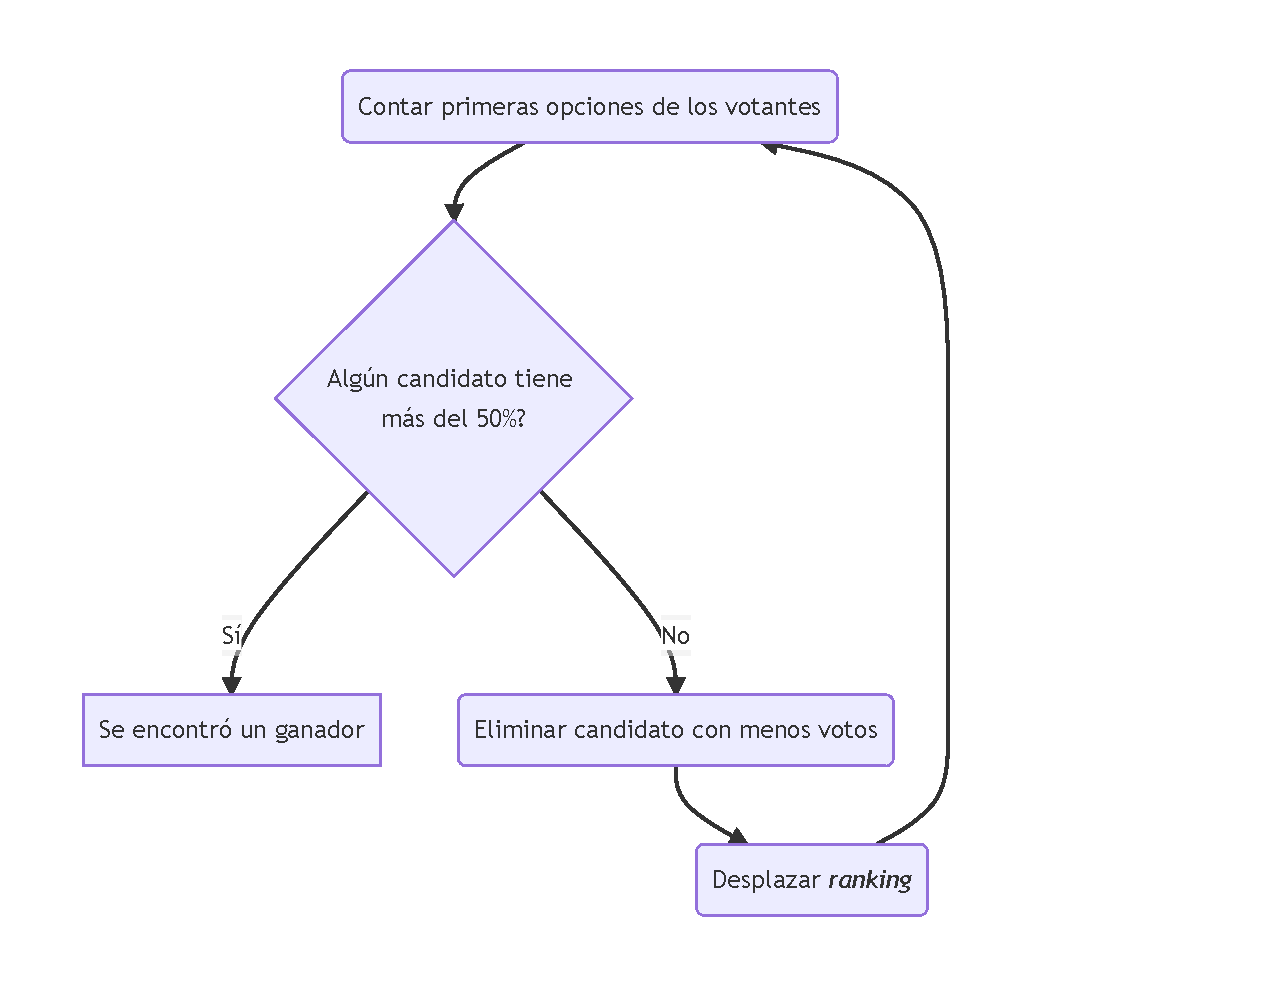
\includegraphics[width=0.8\textwidth]{Graphics/irv.pdf}
    \caption{Diagrama de flujo del m\'etodo de desempate instant\'aneo.}
    \label{fig:irv}
\end{figure}